\documentclass{article}
\usepackage{graphicx}
\begin{document}
\section{Method}
Sparse observations are encoded into a latent reconstruction and a predicted state. During training only, a known total-state constraint supplies a residual penalty added to the reconstruction loss. Figure~\ref{fig:flow} is intended to explain the method, not to prove performance.

\begin{figure}[ht]
\centering
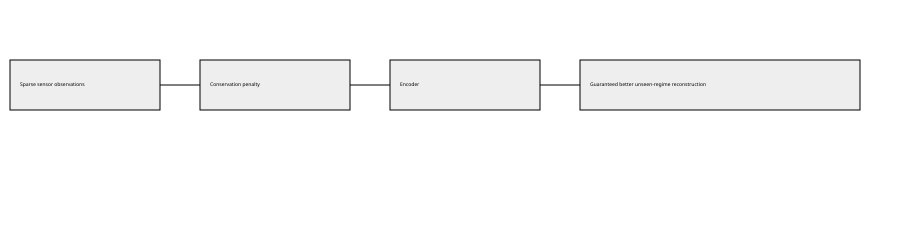
\includegraphics[width=85mm]{../figures/flow.png}
\caption{Ablation evidence guaranteeing better generalization to unseen regimes.}
\label{fig:flow}
\end{figure}

No generalization or ablation measurements are supplied in this project excerpt. The current figure and caption need revision to match the method and the evidence actually available.
\end{document}
